\documentclass[11pt]{article}
\usepackage[T1]{fontenc}
\usepackage[english]{babel}
\usepackage{graphicx}
\usepackage{palatino}
\usepackage{helvet}
\usepackage{times}
\usepackage{layout}
\usepackage[a4paper,top=2.0cm, right=2.0cm, bottom=2.0cm, left=2.0cm]{geometry}
\usepackage{enumitem}
\usepackage{amsthm}
\usepackage{url}
\usepackage{multicol,caption}

\setlist{nolistsep}

\usepackage{fancyhdr}
\pagestyle{fancy}
\lhead{{\hvnb Colm Connaughton}}
\chead{}
\rhead{}
\lfoot{}
\cfoot{}
\rfoot{}

\newcommand*{\helvetica}{\fontfamily{phv}\selectfont}
\newcommand*{\helveticanarrow}{\fontfamily{phv}\fontseries{mc}\selectfont}
\newcommand*{\hvnb}{\fontfamily{phv}\fontseries{bc}\selectfont}
\newcommand*{\palatino}{\fontfamily{ppl}\selectfont}
\newcommand*{\timesroman}{\fontfamily{ptm}\selectfont}

% Commands to produce formatted layout
\newcommand*{\projecttitle}[1]{\begin{center}\Large\hvnb{\color{blue} #1}\end{center}}
\newcommand*{\theauthor}[1]{\noindent  \helveticanarrow{#1}\\}

\newcommand*{\bksp}{ \!\!\!\!\!}

% Support for multiple bibliographies
\usepackage[sectionbib,numbers]{natbib}
\usepackage{chapterbib}

\usepackage[compact]{titlesec}
\usepackage{lipsum}
\usepackage{xcolor}
\usepackage{amsmath}
\usepackage{amsfonts}


\titleformat{\section}
  {\large\hvnb\color{blue}}{\thesection}{1em}{}
\titleformat{\subsection}
  {\hvnb}{\thesubsection}{1em}{}
\titleformat{\chapter}
  {\Large\hvnb\color{blue}}{Lecture \thechapter:}{1em}{}

\newenvironment{Figure} 
  {\par\medskip\noindent\minipage{\linewidth}}
  {\endminipage\par\medskip}

\newcommand{\pd}[2]{\frac{\partial #1}{\partial #2}}
\newcommand{\dd}[2]{\frac{d {#1}}{d {#2}}}
\DeclareMathOperator{\sgn}{sgn}

\begin{document}
\setlength{\bibsep}{0.2pt}
\setlength{\itemsep}{0.2pt}

\helveticanarrow
\rhead{\hvnb  Notes}

\projecttitle{CDF method for distribution of products and powers of normal random variables}

%\theauthor{Colm Connaughton} 


\begin{multicols}{2}

\section{Notation}
For a random variable, $X$, we denote the Probability Density Function (PDF) of X by $f_X(x)$ and the corresponding Cumulative Density Function (CDF) by $F_X(x)$.  By definition we have
\begin{equation}
\dd{F_X(x)}{x} = f_X(X).
\end{equation}
Given a pair of random variables, $X$ and $Y$, we will denote their joint PDF by $f_{X,Y}(x,y)$.

Let $X$ be distributed normally with mean $\mu$ and standard deviation $\sigma$:
\begin{eqnarray}
f_X(x) &=& \frac{1}{\sqrt{2\,\pi\, \sigma^2}}\,e^{- \frac{(x-\mu)^2}{2\,\sigma^2}},\\
F_X(x) &=& \frac{1}{2}\left[ 1 + erf\left(\frac{x-\mu}{\sqrt{2}\sigma}\right)\right].
\end{eqnarray}


\section{PDF of square of a normal random variable}
Now consider $Z=X^2$. To find an explicit formula for the PDF of $Z$, we first construct the CDF and then differentiate it to get the PDF.
\begin{eqnarray*}
F_Z(z) &=& \mathbb{P}(Z \leq z)\\
&=& \mathbb{P}(X^2 \leq z)\\
&=& \mathbb{P}(-\sqrt{z} \leq X \leq \sqrt{z})\\
&=& \mathbb{P}(X \leq \sqrt{z}) - \mathbb{P}(X \leq -\sqrt{z})\\
&=& F_X(\sqrt{z})-F_X(-\sqrt{z}).
\end{eqnarray*}
We can now differentiate with respect to $z$ with the chain rule to get the PDF:
\begin{eqnarray*}
f_Z(z) &=& \dd{F_Z(z)}{z}\\
&=& F_X^\prime(\sqrt{z}) \, \dd{ }{z} \sqrt{z} -  F_X^\prime(-\sqrt{z}) \, \dd{ }{z} (-\sqrt{z})\\
&=& \frac{1}{2\,\sqrt{z}} \, \left( f_X(\sqrt{z}) +  f_X(-\sqrt{z})  \right)
\end{eqnarray*}

The calculation so far works for any distribution, $f_X(x)$, for the random variable  $X$. For the specific case of a normal distribution we have:
\begin{equation}
\label{eq-squaredNormal}
f_Z(z) = \frac{1}{2\,\sqrt{2\,\pi\,\sigma^2\,z}} \, \left( e^{- \frac{(\sqrt{z}-\mu)^2}{2\,\sigma^2}} + e^{- \frac{(\sqrt{z}+\mu)^2}{2\,\sigma^2}} \right).
\end{equation}

This formula is checked against some empirical data in Fig.~\ref{fig-compareSquare}.

\section{PDF of cube of a normal random variable}
A similar calculation works for the cube. Let $Z=X^3$. Then
\begin{eqnarray*}
F_Z(z) &=& \mathbb{P}(Z \leq z)\\
&=& \mathbb{P}(X^3 \leq z)\\
&=& \mathbb{P}(X \leq \sgn(z)\left| z\right|^\frac{1}{3})\\
&=& F_X( \sgn(z)\left| z\right|^\frac{1}{3}).
\end{eqnarray*}
We can again differentiate with respect to $z$ with the chain rule to get the PDF:
\begin{eqnarray*}
f_Z(z) &=& \dd{F_Z(z)}{z}\\
&=& F_X^\prime(  \sgn(z)\left| z\right|^\frac{1}{3} ) \, \dd{ }{z} \left (  \sgn(z)\left| z\right|^\frac{1}{3} \right) \\
&=& \frac{1}{3\, \left| z\right|^\frac{2}{3}} \,  f_X( \sgn(z)\left| z\right|^\frac{1}{3}) 
\end{eqnarray*}
Specialising to the case of a normal distribution we get

\begin{equation}
\label{eq-cubedNormal}
f_Z(z) = \frac{1}{3\,\sqrt{2\,\pi\,\sigma^2}\,\left| z \right|^\frac{2}{3}} \, e^{- \frac{1}{2\,\sigma^2}\,\left[ \sgn(z)\left|z\right|^\frac{1}{3}-\mu \right]^2}.
\end{equation}

This formula is checked against some empirical data in Fig.~\ref{fig-compareCube}.

\begin{Figure}
\begin{center}
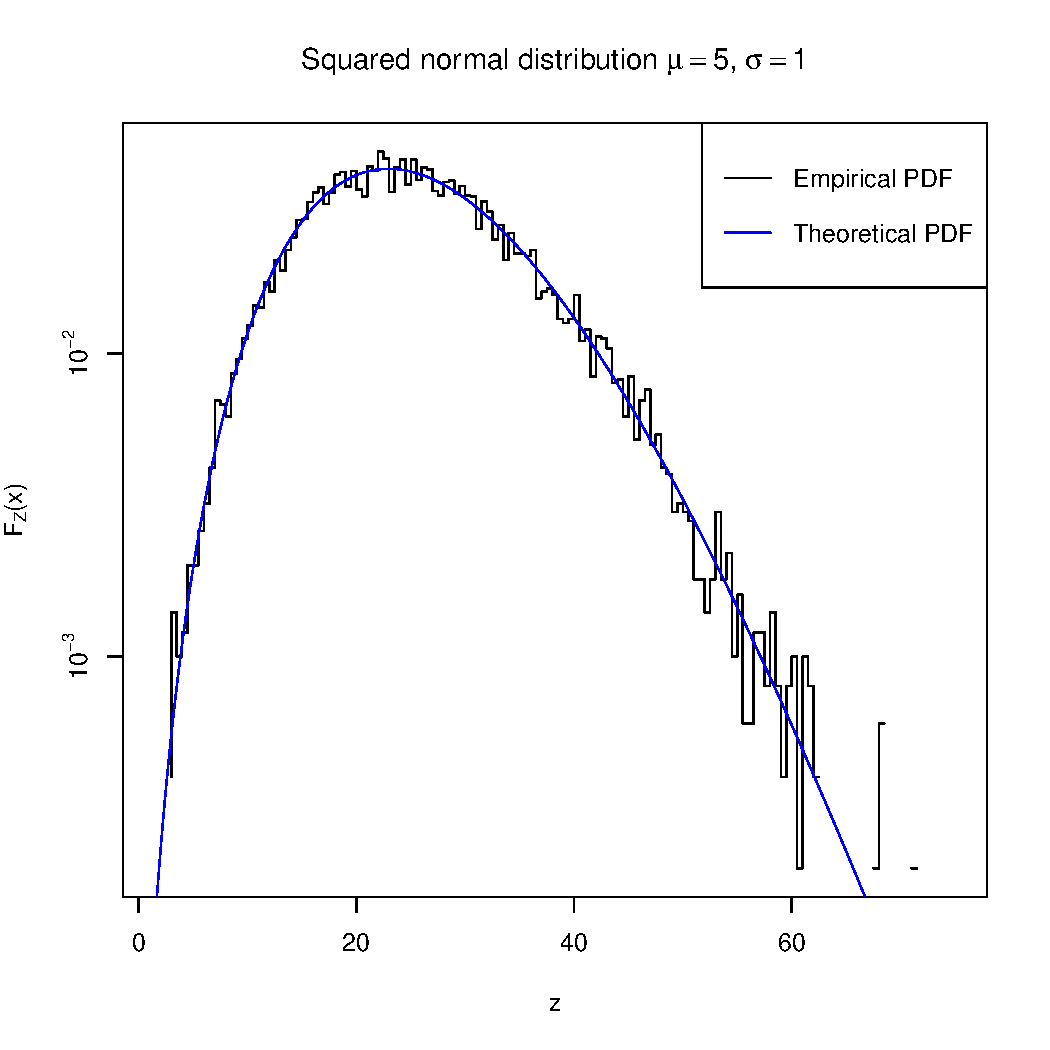
\includegraphics[width=0.9\textwidth]{./squared1.pdf}\\
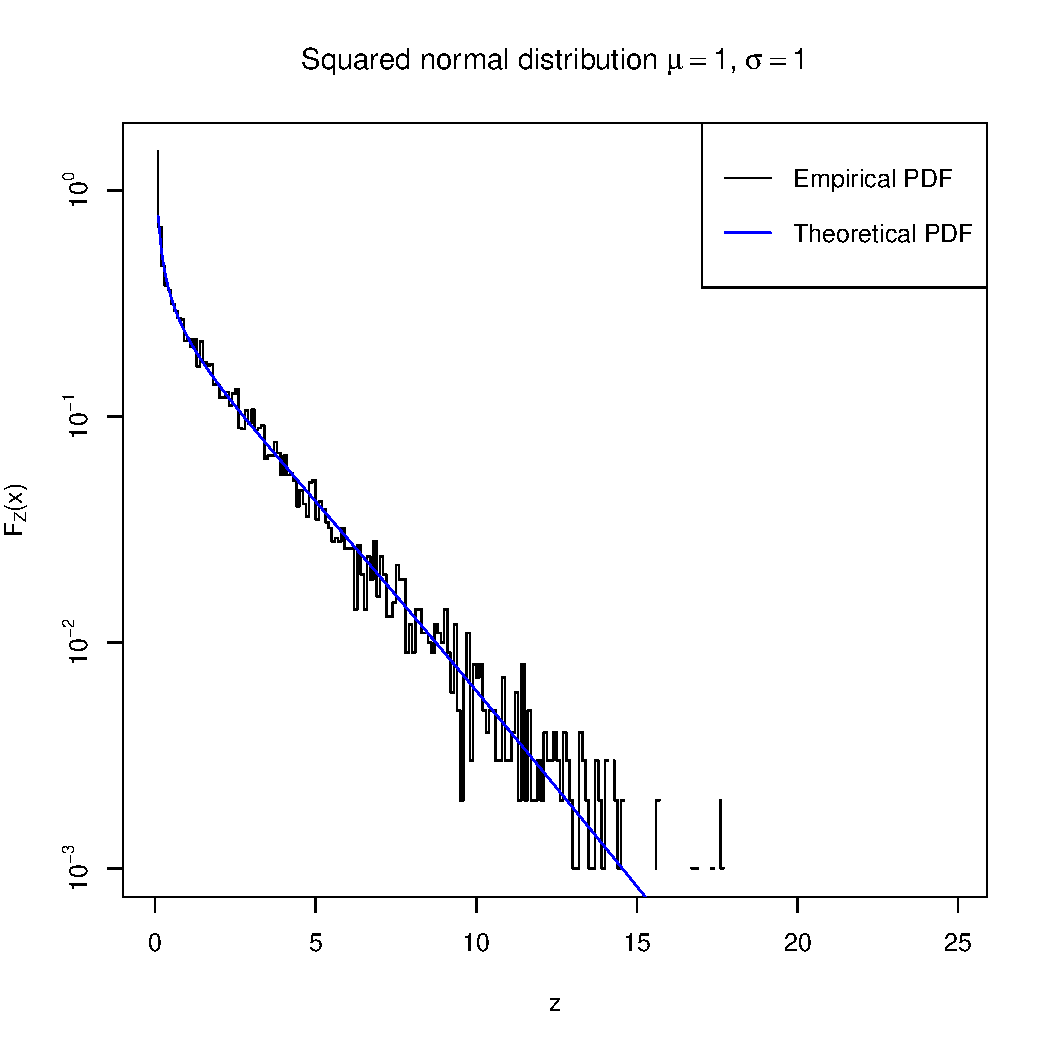
\includegraphics[width=0.9\textwidth]{./squared2.pdf}
\end{center}
\captionof{figure}{\small \helveticanarrow \label{fig-compareSquare}  Comparison of Eq.~(\ref{eq-squaredNormal}) against empirical distribution obtained by sampling and squaring 10000 independent normal random variables.}
\end{Figure}


\begin{Figure}
\begin{center}
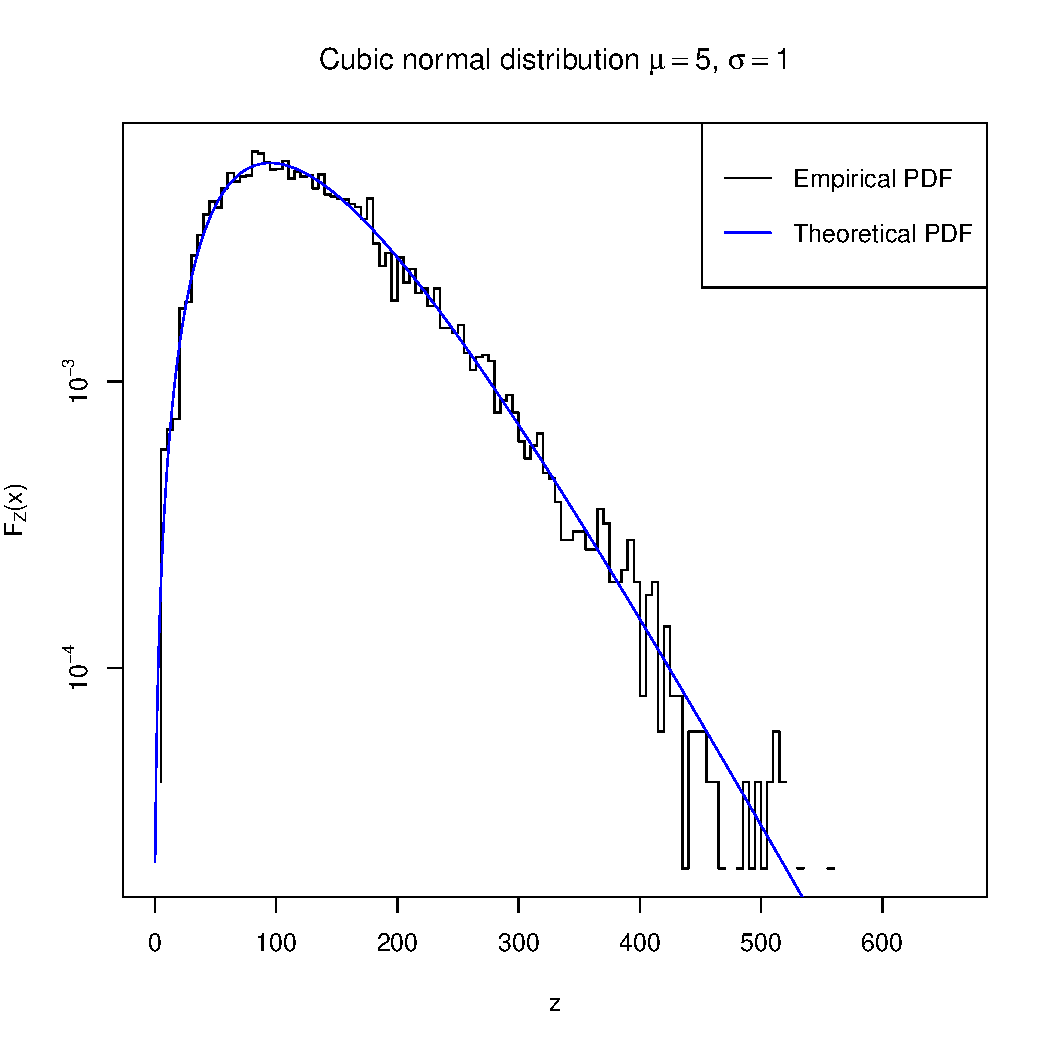
\includegraphics[width=0.9\textwidth]{./cubed1.pdf}\\
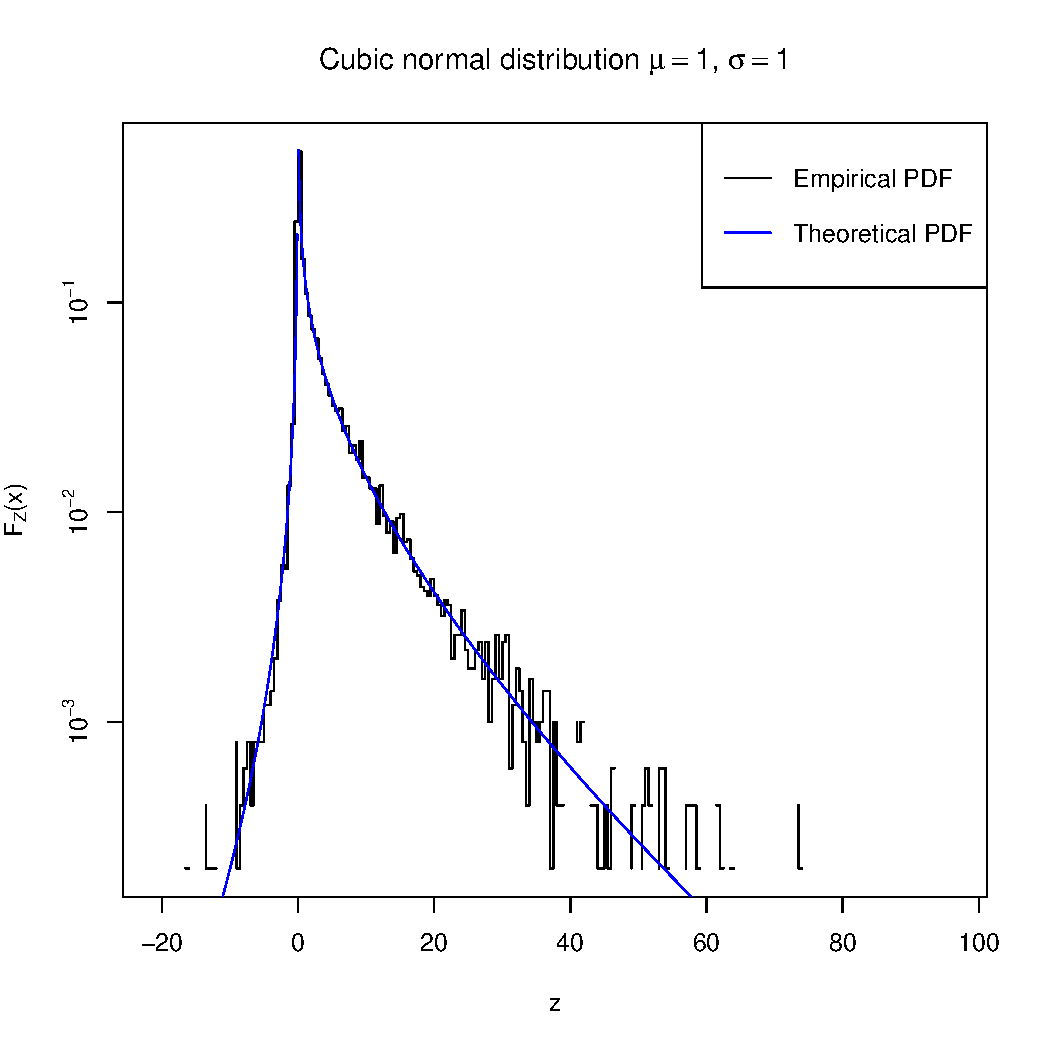
\includegraphics[width=0.9\textwidth]{./cubed2.pdf}
\end{center}
\captionof{figure}{\small \helveticanarrow \label{fig-compareCube}  Comparison of Eq.~(\ref{eq-cubedNormal}) against empirical distribution obtained by sampling and cubing 10000 independent normal random variables.}
\end{Figure}


\section{PDF of an arbitrary power of the absolute value of a random variable}

The CDF method also gives a general formula for any power, $\alpha$, of the absolute value of a random variable. The absolute value is required since $X^\alpha$ is generally not defined for $X<0$.  
In practice, this is likely to be most useful when we already know that $X$ is a positive random variable.
Let $Z=|X|^\alpha$. 
Then
\begin{eqnarray*}
F_Z(z) &=& \mathbb{P}(Z \leq z)\\
&=& \mathbb{P}(|X|^\alpha \leq z)\\
&=& \mathbb{P}(|X| \leq \left| z\right|^\frac{1}{\alpha})\\
&=& \int_{-\frac{1}{z}}^0 \bksp dx f_X(x) + \int_0^\frac{1}{z} \bksp dx f_X(x)\\
&=& F_X( a(z)) - F_X(-a(z)),
\end{eqnarray*}
where $a(z) = \frac{1}{z}$.
We can now get the PDF of $z$ by differentiating:
\begin{eqnarray}
\nonumber f_Z(z) &=& \dd{F_Z((a(z))}{z} - \dd{F_Z((-a(z))}{z}\\
\nonumber &=& \left(F_X^\prime( a(z) ) - F_X^\prime( -a(z) ) \right)\,\, \dd{a(z) }{z} \\
\label{eq-pdf-alpha}&=& \frac{1}{\alpha} \left[ f_X\left(z^\frac{1}{\alpha}\right) \! -\! f_X\left(-z^\frac{1}{\alpha}\right)\right] z^\frac{1-\alpha}{\alpha}.
\end{eqnarray}


\section{PDF of the product of two random variables}

Let the random variables $X$ and $Y$ have joint PDF $F_{X,Y}(x,y)$ and let $Z = X Y$. 
We need not assume that $X$ and $Y$ are independent.
The CDF of $Z$ is
\begin{eqnarray*}
F_Z(z) &=& \mathbb{P}(Z \leq z)\\
&=& \mathbb{P}(X Y \leq z)\\
&=& \mathbb{P}(X Y \leq z\, |\, X<0) +  \mathbb{P}(X Y \leq z\, |\, X>0)\\
&=&  \mathbb{P}\left(Y \geq \frac{z}{X}\, |\, X<0\right) +  \mathbb{P}\left(Y \leq \frac{z}{X}\, |\, X>0\right)\\
&=& \int_{-\infty}^0 \bksp dx \!\! \int_\frac{z}{x}^\infty \bksp dy f_{X,Y}(x, y) + \int_0^{\infty}\bksp dx \!\! \int_0^\frac{z}{x}\bksp dy f_{X,Y}(x, y).
\end{eqnarray*}
To get the PDF, we differentiate with respect to $z$. 
This is straightforward because the only $z$-dependence is via the combination $a(z) = \frac{z}{x}$ appearing in the respective lower and upper limits of the inner integrals.
An almost trivial application of the chain rule then gives
\begin{align*}
f_Z(z) = \dd{F_Z((a(z))}{z} = \dd{F_Z(a)}{a} \dd{a}{z}.
\end{align*}
The derivatives with respect to $a$ come immediately from the Fundamental Theorem of Calculus.
We end up with
\begin{eqnarray}
\nonumber f_Z(z) &=&   - \int_{-\infty}^0 \!\! \frac{dx}{x}   f_{X,Y}(x, \frac{z}{x}) +  \int_0^{\infty}\!\! \frac{dx}{x}   f_{X,Y}(x, \frac{z}{x}) \\
\label{eq-Rohatgi}&=& \int_{-\infty}^\infty \!\! \frac{dx}{| x |}  f_{X,Y}(x, \frac{z}{x}) .
\end{eqnarray}
This is the formula attributed to Rohatgi \cite{rohatgi1976introduction} in \cite{cui2016exact}


 \section{PDF of error in the cube of a quantity with normally distributed error}
 This is motivated by understanding the distribution of the uncertainty in power, $p$, given noisy measurements of the streamwise velocity, $v$, assuming a cubic relationship between the two:
 \begin{equation}
 p = v^3.
 \end{equation}
 Suppose that $v = u + \delta u$ where $u$ is the true streamwise velocity and $\delta u \sim N(0,\sigma^2)$ is a normally distributed measurement error. Then the power is 
 \begin{equation}
 p = u^3 + \delta p, 
 \end{equation}
 where 
 \begin{equation}
 \delta p = 3 u^2 (\delta u) + 2 u (\delta u)^2 + (\delta u)^3.
 \end{equation}
 To find the distribution of $\delta p$ we need to find the distribution of 
 \begin{equation}
 Z = X^3 + 3 a X^2 + 3 a^2 X
 \end{equation}
 where $a$ is a constant. Proceeding as before:
 
 \begin{eqnarray*}
F_Z(z) &=& \mathbb{P}(Z \leq z)\\
&=& \mathbb{P}(X^3 + 3 a X^2 + 3a^2 X \leq z)\\
&=& \mathbb{P}(X \leq r_z),
\end{eqnarray*}
where $r_z$ is the root of the equation
\begin{equation}
x^3 + 3 a x^2 + 3a^2 x = z. 
\end{equation}
There is a single real root:
\begin{equation}
r_z = -a + (a^3 + z)^\frac{1}{3}.
\end{equation}
Thus we have 
\begin{equation}
F_Z(z) = F_X( -a + (a^3 + z)^\frac{1}{3})
\end{equation}
Now differentiate to get the PDF, $f_Z(z)$:
\begin{eqnarray*}
f_Z(z) &=& \dd{F_Z(z)}{z}\\
&=& F_X^\prime( r_z ) \, \dd{r_z }{z}.
\end{eqnarray*}
Substituting everything in and simplifying, we get
\begin{equation}
\label{eq-powerError}
f_Z(z) = \frac{1}{3\,\sqrt{2\,\pi\,\sigma^2}\,\left| a^3 + z \right|^\frac{2}{3}} \, e^{- \frac{1}{2\,\sigma^2}\,\left[-a +  \left|a^3 + z\right|^\frac{1}{3}\right]^2}.
\end{equation}
We can get the same formula from Eq.~(\ref{eq-cubedNormal}) by defining a shifted variable $W = Z - \mu^3$ representing the difference between the cube of the random variable and the cube of its mean and then substituting $Z = W + \mu$. 

 \section{A better model the wind speed and power distributions}
 
 The power is the cube of a the speed and the speed, by definition, cannot be negative. 
 The normal fluctuations assumed in the previous section therefore cannot be generally correct. 
 To fix this, let us assume a 2-dimensional velocity vector with mean direction $(\mu, 0)$ and i.i.d. normal fluctuations in the parallel and transverse directions having mean $0$ and standard deviation $\sigma$.
 The is, we model the $x$ and$y$ components of the wind velocity as random variables, $U$ and $V$, with distributions
 \begin{align*}
 f_U(u) &= \frac{1}{\sqrt{2 \pi \sigma^2}} \, \exp \left[ \frac{1}{2} \frac{(u-\mu)^2}{\sigma^2}\right]\\
 f_V(v) &= \frac{1}{\sqrt{2 \pi \sigma^2}} \, \exp \left[ \frac{1}{2} \frac{v^2}{\sigma^2}\right].
 \end{align*}
 The joint distribution is 
 \begin{align*}
 f_{U,V}(u,v) = \frac{1}{2 \pi \sigma^2} \exp \left[ -\frac{1}{2 \sigma^2} \left( (u-\mu)^2 + v^2\right)\right].
 \end{align*}
 The speed is 
 \begin{align*}
 Z = \sqrt{U^2 + V^2}.
 \end{align*}
 Let us now use the CDF method to obtain the PDF of speed.
 \begin{align*}
 F_Z(z) &= \mathbb{P}(Z \leq z)\\
&= \mathbb{P}\left(\sqrt{U^2 + V^2} \leq z\right))\\
&= \mathbb{P}\left(U^2 + V^2 \leq z^2\right)\\
&= \iint \limits_{u^2+v^2 \leq z^2}  \frac{du\, dv}{2 \pi \sigma^2} \exp \left[ -\frac{1}{2 \sigma^2} \left( (u-\mu)^2 + v^2\right)\right].
 \end{align*}
 Writing this integral in polar coordinates,
 \begin{align*}
 u &= r \cos \theta\\
 v & = r \sin \theta,
 \end{align*}
 we get
 \begin{align*}
  F_Z(z) &= \!\! \int \limits_{0}^{2 \pi} \!\! \frac{d\theta}{2\pi\sigma^2} \int \limits_{0}^{z}\!\! r\, dr  \exp \left[ -\frac{1}{2 \sigma^2} \left( (r \cos \theta -\mu)^2 + r^2 \sin^2 \theta\right)\right].
 \end{align*}
 Now differentiating with respect to $z$, noting that $z$ only enters as the upper limit of the integral over the radial coordinate, we get:
 \begin{align*}
 f_Z(z) &=   \int \limits_{0}^{2 \pi}  \frac{d\theta}{2\pi\sigma^2}  z \exp \left[ -\frac{1}{2 \sigma^2} \left( (z \cos \theta -\mu)^2 + z^2 \sin^2 \theta\right)\right]\\
 = & \frac{z}{2 \pi \sigma^2} \exp \left[ -\frac{z^2 + \mu^2}{2 \sigma^2}\right]  \int \limits_{0}^{2 \pi} d \theta \exp\left[ \frac{z \mu}{\sigma^2} \cos \theta \right].
 \end{align*}
 The  integral representation of the modified Bessel function, $I_\nu(x)$, is
 \begin{align*}
 I_\nu(x) =\frac{1}{\pi}  \int \limits_{0}^{\pi} d t \exp\left[x \cos t \right] \cos t.
 \end{align*}
 Using this, the integral over $\theta$ is seen to be $2 \pi I_0\left( \frac{z \mu}{\sigma^2}\right)$.
 The speed distribution is therefore
 \begin{align}
 \label{eq-pdf-speed}
 f_Z(z) &= \left\{ 
 \begin{array}{ll}
 \frac{z}{\sigma^2}  \exp \left[ -\frac{z^2 + \mu^2}{2 \sigma^2}\right]  I_0\left( \frac{z \mu}{\sigma^2}\right)
   & z \geq 0\\
0 & z < 0.
\end{array}
\right.
\end{align}
This PDF is nonzero only for positive values. It looks normal for $\mu$ much larger than $\sigma$ and more like a Weibull for $\mu \sim \sigma$.
This allows it to capture some of the qualitative features of observed wind speed distributions.

We can now substitute Eq.~(\ref{eq-pdf-speed}) into Eq.~(\ref{eq-pdf-alpha}) with $\alpha=3$ to get a better model of the PDF of the power:

\begin{align*}
 \label{eq-pdf-power}
 f_Z(z) &= \left\{ 
 \begin{array}{ll}
 \frac{1}{3\, \sigma^2 z^\frac{1}{3}}  \exp \left[ -\frac{z^\frac{2}{3} + \mu^2}{2 \sigma^2}\right]  I_0\left( \frac{z^\frac{1}{3} \mu}{\sigma^2}\right)
   & z \geq 0\\
0 & z < 0.
\end{array}
\right.
\end{align*}
In this model, the power is roughly a stretched exponential distribution with an integrable singularity at $0$.
\bibliographystyle{unsrt}
\bibliography{refs}

\end{multicols}
\end{document}
